\section{State-of-the-Art}
\label{sec:sota}


Den Straßenverkehr theoretisch abzubilden, ist fachübergreifend eine große Herausforderung in der Forschung.
Hier ergeben sich u. a. Aufgaben im Bereich der Mathematik (Routenplanung z. B. durch graphentheoretische Ansätze), Psychologie (Erforschung menschlichen Verhaltens) und nicht zuletzt Informatik (Simulationen).

Die Simulation von Fahrverhalten ist aufgrund des unsicheren Faktors Mensch, der als Haupt"-entscheider nur durch Wahlmöglichkeiten mit vorgegebenen unterschiedlich hohen Wahrscheinlichkeiten modelliert werden kann, ein Bereich in dem seit den 1930er Jahren geforscht wird.

\cite{genealogy}\sa{nicht mit einer Referenz den Satz beginnen} gibt einen umfassenden Überblick über die verschiedenen Ansätze (siehe \cref{figure:family-tree}), die seit den ursprünglichen Annahmen der \enquote{fundamental relation} von Bruce D. Greenshields (1934/35), dass es einen Zusammenhang zwischen dem Abstand zwischen Fahrzeugen ($s$, genauer zweier Fahrzeugfronten) und deren Geschwindigkeit ($v$) geben muss, verfolgt wurden. 
\begin{figure}[hptb]
 \centering
 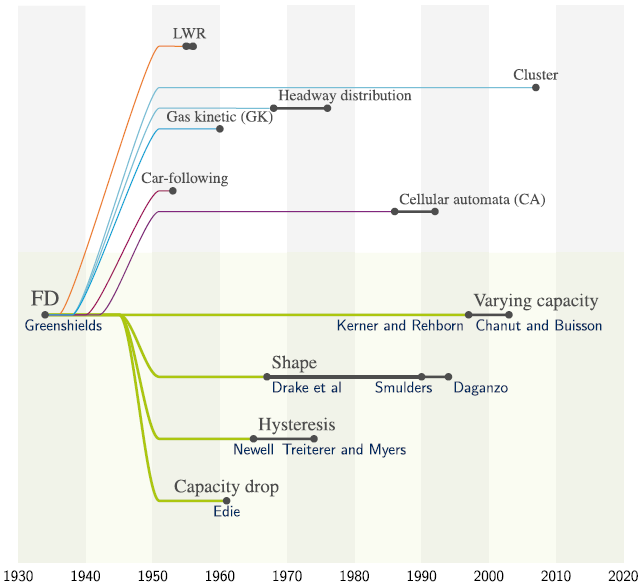
\includegraphics[width=0.9\textwidth]{family-tree}
 \caption[Überblick über die Entwicklung der Verkehrsflussmodelle]
 		{\enquote{Stammbaum} der Verkehrsflussmodelle, aus \cite{genealogy}}
 \label{figure:family-tree}
\end{figure}
\noindent
Die Fundamentalrelation, heute bekannt als Fundamentaldiagramm, kann aber auch mit Hilfe anderer Variablen, wie z. B. der Verkehrsdichte ($\rho$, der durchschnittlichen Anzahl von Fahrzeugen auf einer bestimmten Strecke) und dem Verkehrsfluss ($q$, der durchschnittlichen Anzahl von Fahrzeugen pro Zeiteinheit) wiedergegeben werden, siehe \cref{figure:fundamental-relations}. 
\begin{figure}[hptb]
 \centering
 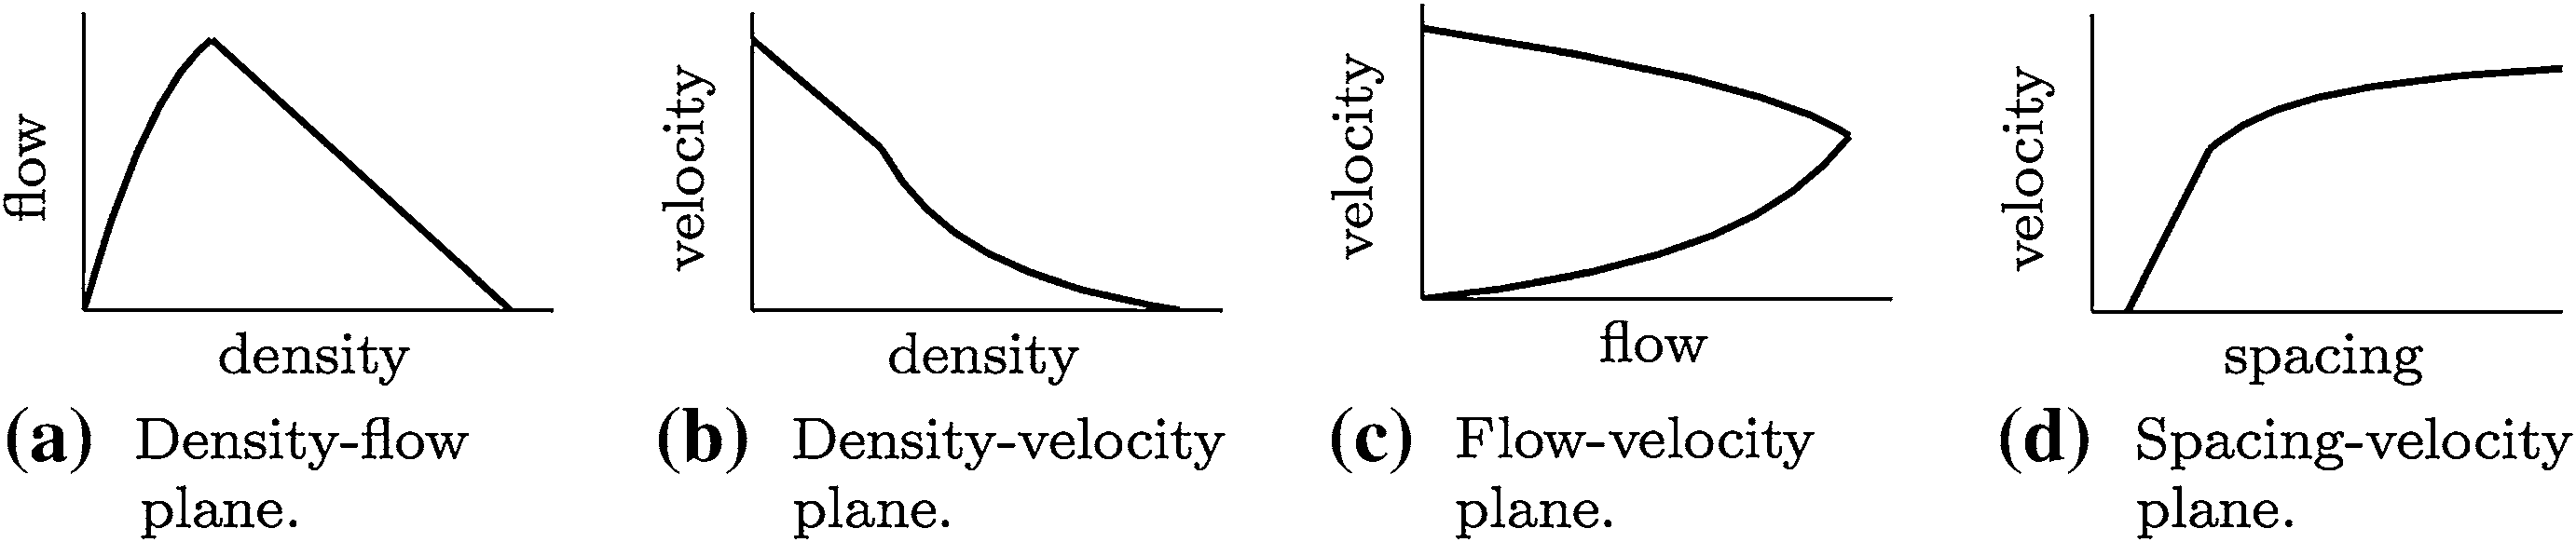
\includegraphics[width=0.9\textwidth]{fundamental-relations}
 \caption[Fundamentalrelationen in verschiedenen Ebenen]
 		{Fundamentalrelationen in verschiedenen Ebenen, aus \cite{genealogy}}
 \label{figure:fundamental-relations}
\end{figure}

Verschiedene Ansätze, Verkehrsflüsse zu simulieren, die auch unterschiedliche Sichtweisen auf Verkehr und Verkehrsteilnehmer verfolgen, %- mikro- makro- und mesoskopisch, 
wurden und werden verfolgt, vgl. \cite{dingding}.
\begin{itemize}
	\item \textit{Mikroskopische Modelle} simulieren einzelne Fahrzeug-Fahrer-Einheiten, basierend auf dem Fahrerverhalten. Zwei Modellierungsansätze können hier unterschieden werden: das Fahrzeugfolgemodell (\enquote{car-following model}) und das Zellularautomatenmodell. Zu letzterem später mehr.
	\item \textit{Makroskopische Modelle}  konzentrieren sich auf Charakteristiken des Verkehrsflusses, wie mittlere Geschwindigkeit (\enquote{average velocity}), Verkehrsdichte, -fluss und Durchschnittsgeschwindigkeit des Verkehrsstromes (\enquote{mean speed of a traffic stream}).
	\item \textit{Mesoskopische Modelle} kombinieren die beiden vorgenannten Modelle, simulieren die Fahrzeuge einzeln, nutzen aber die makroskopische Sicht, um deren Aktivitäten und Interaktionen zu beschreiben. Ein klassischer Vertreter ist das gaskinetische Modell.
\end{itemize}



\subsection{Zellularautomaten}
%\addcontentsline{toc}{subsection}{Zellularautomaten}
\label{sec:ca}

Zellularautomaten werden seit etwa 25-30 Jahren für die Verkehrssimulation verwendet.

\begin{quote}
Ein zellulärer Automat ist eine regelmäßige Annordnung von Zellen. Jede Zelle kann eine endliche Zahl von Werten / Zuständen annehmen und hat eine  begrenzte Zahl von Nachbarzellen, die sie beeinflussen können. Das Muster des gesamten zellulären Automaten ändert sich in einzelnen Schritten, die durch eine Reihe von Übergangsregeln bestimmt werden, die für alle Zellen gelten. (aus \cite{cell-autom})
\end{quote} 

\noindent
Vereinfacht kann eine Fahrspur einer Straße als Aneinanderreihung vieler Zellen gesehen werden(siehe \cref{figure:grid-umgebung}) und damit durch den Zellularautomaten abgebildet werden. 
\begin{figure}[hptb]
 \centering
 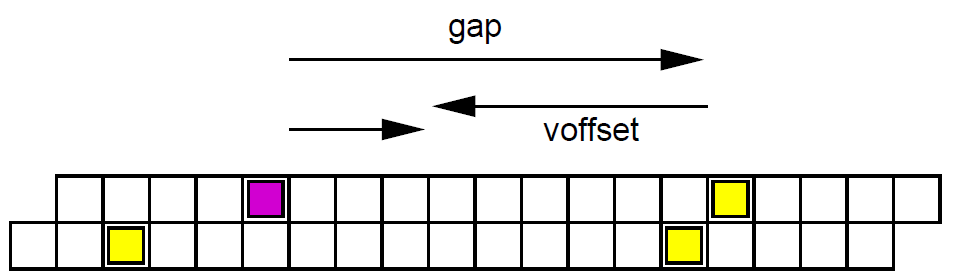
\includegraphics[width=0.9\textwidth]{grid-umgebung}
 \caption[Beispiel für eine Griddarstellung einer Straße]
 		{symbolische Griddarstellung einer Straße mit zwei Fahrspuren mit Fahrzeugen, aus \cite{multi-lane}}
 \label{figure:grid-umgebung}
\end{figure} \sa{einspurig croppen, obere Zeile und Richtungspfeil belassen}
Dies führt schließlich zu einer gridbasierten Simulationsumgebung. 


\subparagraph{Das Nagel-Schreckenberg-Modell}
%\subsubsection*{Das Nagel-Schreckenberg-Modell}
%\addcontentsline{toc}{subsubsection}{Das Nagel-Schreckenberg-Modell}
%\label{sec:na-sch}

Nagel und Schreckenberg war es 1992 gelungen, auf Basis solcher Automaten mit einfachen Regeln das mikroskopische Verhalten jedes Fahr\-zeug\-füh\-rers so abzubilden, dass sich die makroskopische Sicht auf den Verkehrsfluss als für Autobahnverkehr realistisch darstellte. 
Jedes Fahrzeug durchläuft in jedem Zeitschritt die folgenden Übergangsregeln, vgl. \cite{na-sch}. 

\begin{enumerate}
	\item \textit{Beschleunigung}: Solange ein Fahrzeug nicht seine max. Geschwindigkeit $v_{max}$ (Zellen/""Zeitschritt) erreicht hat und ein vorausfahrendes Fahrzeug weit genug entfernt ist, erhöht es die Geschwindigkeit um $1$, $v \rightarrow v+1$;
	\item \textit{Abbremsen}: Hat ein Fahrzeug ein anderes Fahrzeug $j$ Zellen vor sich, dann reduziert es die Geschwindigkeit auf $j-1$, $v \rightarrow j-1$;
	\item Zufallsgröße, auch \textit{\enquote*{Trödelwahrscheinlichkeit}}: Mit einer Wahrscheinlichkeit $p$ wird die Geschwindigkeit ($v > 0$) eines Fahrzeuges um $1$ reduziert, $v \rightarrow v-1$;
	\item \textit{Fahrzeugbewegung}: Jedes Fahrzeug wird um $v$ Zellen nach vorn gesetzt.
\end{enumerate}

\noindent
Erstmals konnte das Entstehen von \enquote{Stau aus dem Nichts} und das Vorhandensein von \enquote{Stauwellen}, die sich rückwärts durch einen solchen Stau bewegen, simulatorisch dargestellt werden.

Die Rechenumgebung wurde als eindimensionales Array mit $L$ Zellen definiert, $L$ ist dabei eine ganze Zahl. 
Jede der Zellen kann entweder von einem Fahrzeug belegt oder frei sein. 
Eine Simulation in dieser Grid-Welt hat den Vorteil, dass die Erkenntnisse auf die reale Welt skaliert werden können. 
Es wurde eine Zelllänge von 7,5\nolinebreak[4] m angenommen (vgl. \cite[S. 2227]{na-sch}), was ungefähr dem beanspruchten Platz eines Pkw - von Fahrzeugfront zu Fahrzeugfront - in einer Stausituation entspricht (Fahrzeuglänge + Abstand). 
Jedes Fahrzeug hat eine ganzzahlige Geschwindigkeit zwischen null und $v_{max}$.

\begin{table}[ht]
\begin{center}
\setlength{\tabcolsep}{0.5em} % for the horizontal padding
{\renewcommand{\arraystretch}{1.2}% for the vertical padding
\begin{tabular}{| c | c | c |}
\hline 
$v^{sim}$ in $\frac{\text{Zellen}}{\text{Zeitschritt}}$ & $\widehat{=}$ $v^{real}$ in $\frac{m}{s}$ & $=$ in $\frac{km}{h}$ \\ \hline 
$1$ & 7,5 & 27 \\ \hline
$2$ & 15 & 54 \\ \hline
$3$ & 22,5 & 81 \\ \hline
$4$ & 30 & 108 \\ \hline
$5$ & 37,5 & 135 \\ \hline
$6$ & 45 & 162 \\ \hline
\end{tabular}
}
\caption{Umrechnung Geschwindigkeiten Gridwelt $\rightarrow$ reale Welt}
\end{center}
\label{tab:umrechnung-zelle-kmh}
\end{table}

Zu Beginn eines Simulationslaufes wurden $N$ Fahrzeuge zufällig auf die $L$ Zellen verteilt.
Dies führte dazu, dass über den Durchlauf hinweg eine konstante Fahrzeugdichte $\rho$ im System garantiert werden konnte:
\begin{equation}
\rho = \dfrac{N}{L} = \dfrac{\text{Anzahl der Fahrzeuge im System}}{\text{Anzahl der Zellen des Systems}}
\nonumber
\end{equation}

\noindent
Die Simulation erfolgte unter Nutzung periodischer Randbedingungen. 
Wie in \cite[Abb. 1.5]{peri-rand} für die Umgebung von Pixeln\sa{bitte mal kontrollieren, ob man wirklich von Pixeln hier spricht, denn Pixel ist ein Element aus der Computergraphik, ein Fahrzeug in dem Bild ist aber mehr als ein Pixel} beschrieben, werden die Fahrzeuge somit vom \enquote*{Ende} der Gridstrecke am \enquote*{Anfang} wieder eingesetzt. 
Damit einstand die Möglichkeit einer kontinuierlich arbeitenden Simulationsumgebung, siehe \cref{figure:traffic-simulation}.
\begin{figure}[hptb]
 \centering
 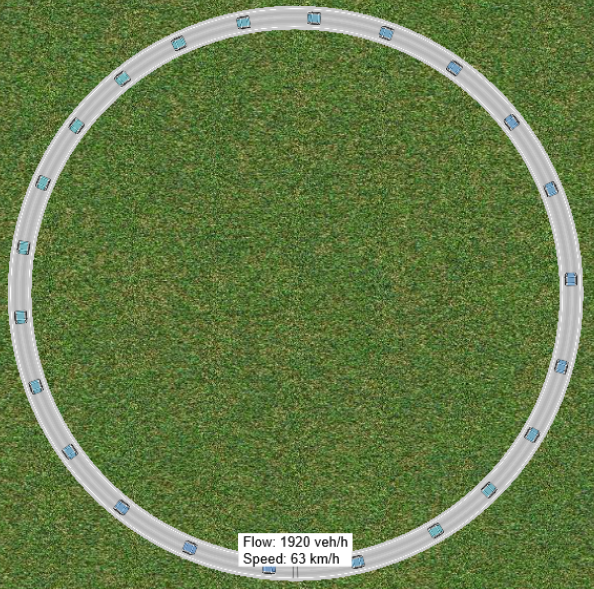
\includegraphics[width=0.5\textwidth]{traffic-simulation}
 \caption[Darstellung des Verkehrs in einem geschlossenen System]
 		{Symbolbild: Verkehr in einem Kreis (geschlossenes System), Screenshot \url{http://traffic-simulation.de}}
 \label{figure:traffic-simulation}
\end{figure} 



\subparagraph{Erweiterung auf Mehrspurigkeit}
%\subsubsection*{Erweiterung auf Mehrspurigkeit}
%\addcontentsline{toc}{subsubsection}{Erweiterung auf Mehrspurigkeit}
%\label{sec:multi-lane}

Um Verkehr auf mehrspurigen Fahrbahnen zu simulieren, war das Originalmodell nicht geeignet. 
1996 folgte deswegen eine Ausdehnung auf Mehrspurigkeit \cite{multi-lane} - zwei Spuren. 
Regeln, die prüfen, ob ein Spurwechsel vorteilhaft ist und einen sicheren, weil kollisionsfreien, und nicht behindernden Spurwechsel ermöglichen, wurden hinzugefügt. Die Regeln 1-3 wurden übernommen. Nach Simulationsläufen, die unerwünschtes Verhalten zeigten, waren die finalen Regeln wie folgt:

\textit{Hinweis:} $\Delta x$ $\widehat{=}$ dem Abstand zum vorausfahrenden Fahrzeug, die Indizes $b$ (\enquote*{behind} - für rückwärtigen Verkehr) und $o$ (\enquote*{other} - für Verkehr auf der Spur auf die gewechselt werden soll) können auch kombiniert werden. 

\begin{itemize}
	\item \textit{Sicherheitsbedingung}: 
	\\	
	die Geschwindigkeit des Fahrzeugs auf der Spur auf die gewechselt werden soll, darf nicht größer als der Abstand des Fahrzeugs sein (keine Behinderung des Nachfolgeverkehrs), $v^{o,b} \leq \Delta x^{o,b}-1$;
	\item \textit{Intention zum Spurwechsel}: 
	\\
	Fahrzeug kann nicht so schnell fahren, wie es möchte, $v_{max} > \Delta x-1$ \\
	UND\\
	die andere Spur ist nicht schlechter als die aktuelle Spur, $\Delta x^{o} \geq \Delta x$
	\item \textit{nach dem Spurwechsel}: 
	\\
	diese Regeln werden mit einer gewissen Wahrscheinlichkeit $p_{l2r}$ (\enquote{Zurückwechselwahrscheinlichkeit}) ausgeführt, \\
	ausreichend großer Abstand zum hinteren Fahrzeug auf der rechten Spur, $v^{o,b}_{max} \leq \Delta x^{o,b}-1$ \\
	UND \\
	ausreichend Platz auf der rechten Spur, $v \leq \Delta x^{o}-1$
\end{itemize}

Wenn es die festgelegten Kriterien zulassen\sa{es wäre sinnvoll genau diese Definition als Grundlage für das erste Mehrspurszenario in der Simulation zu nutzen und sich in der Arbeit darauf zu beziehen}, erfolgt der Spurwechsel auf die linke Spur immer, da dieser nicht an eine Wahrscheinlichkeit geknüpft ist.
Lediglich um die Überbevölkerung der Überholspur zu vermeiden, wurde eine Wahrscheinlichkeit $p_{l2r}$ für das zurückwechseln eingeführt.

Was dieser Modellierung fehlt\sa{und hier genau dann als 'Case Study' für Deine Arbeit zu bezeichnen}, ist die Berücksichtigung irregulärer Verhaltensweisen der Fahrer - Unsicherheiten (z. B. Fehleinschätzungen oder Ängste), Ablenkungen (z. B. Gespräche mit anderen Fahrzeuginsassen, Telefonieren, Suche im Handschuhfach oder nach der fallen gelassenen Zigarette). 

Zusätzlich ist die Bremswirkung, wie auch im ursprünglichen Nagel-Schreckenberg-Modell, \enquote{über\-di\-men\-sio\-niert}. 
Vollbremsungen aus Höchstgeschwindigkeit sind innerhalb kürzester Distanz möglich \cite{acc-free}.
Daraus ergibt sich eine weitere fehlende Komponente der Realität.
Denn auch Unfälle gehören zum Verkehrsgeschehen. \\
Studien zufolge sind drei Viertel der Autofahrer abgelenkt, wenn sie am Steuer sitzen. 
Jeder zehnte Verkehrsunfall in Deutschland wird durch unaufmerksame Autofahrer verursacht. 
In Österreich und der Schweiz geht man, aufgrund der Einordnung in eine eigene Kategorie für diese Art Unfälle, von einer Rate von etwa 30\% der Unfälle mit Personenschäden oder gar Toten aus. (vgl. \cite{dvr-studie})

Laut Statistischem Bundesamt gab es 2016 auf Autobahnen 21193 Unfälle, davon 1435 innerhalb von Baustellen \cite{unf2016}. 
Bei den etwa 13000 km Autobahn \cite{autob2016} entspricht dies durchschnittlich etwa einem Unfall pro 200 km Strecke pro Tag. 
In Wirklichkeit wird es aber Unfallschwerpunkte geben, die diesen Durchschnittswert überschreiten.



\subsection{Stochastische Ansätze}
% \addcontentsline{toc}{subsection}{Stochastische Ansätze}
\label{sec:stochastic-approaches}

Es gibt inzwischen Ansätze, die das mikroskopische Verhalten der Fahrzeugführer aus Realdaten  stochastisch modelliert haben \cite{stoch-carfollow}. 
In den aggregierten Daten wurde eine Laplace-Verteilung der Beschleunigungswerte erkannt. 
Das daraus entwickelte Modell wurde getestet. 
Die Reproduktion der Sicherheitsparameter, wie Zeit bis zur Kollision (TTC, time to collision) und der Bremsrate um einen Unfall zu verhindern (DRAC, deceleration rate to avoid crash) gelang. 
Allerdings konnte das Fundamentaldiagramm nicht nachgestellt werden.

\cite{multi-fuzzy} integriert den Ansatz der Mehrspurigkeit in einem Multiagenten-Fuzzy-System.\sa{genau das ist ein kern meiner Arbeit mit LightJason und das ist in Deiner Arbeit eingebaut} 
Die Spuren werden als Vereinigung mehrerer miteinander kommunizierender einspuriger Zellularautomaten (\enquote{continuous cellular automata}) beschrieben. 
Diese Kommunikation zwischen den Spuren beschränkt sich auf die Sicherheitskriterien, wenn ein Fahrzeug die Spur wechseln möchte. 
Intentionen zum Wechsel zwischen den Spuren werden durch fortwährend aktualisierte \enquote{Stresslevel} je Fahrzeug beeinflusst, die Wahrscheinlichkeiten dafür durch einen Bernoulli-Prozess berechnet.
Dieser Ansatz arbeitet mit Gridzellen und achtet auf Kollisionsfreiheit.



\subsection{Das Social-Force-Vehicle-Modell}
% \addcontentsline{toc}{subsection}{Das Social-Force-Vehicle-Modell}
\label{sec:social-force-vm}

In \cite{dat-ba} wurde mit dem \enquote{Social-Force-Vehicle-Modell} ein neuer Vorschlag für die Simulation von Spurwechseln entwickelt. 
Das Modell orientiert sich bei den Fahrzeugbewegungen an den Grundlagen des Nagel-Schreckenberg-Modells, vermeidet Unfälle aber in erster Linie nicht durch Abbremsen, sondern durch Ausweichen, also Spurwechsel. 

Im Gegensatz zur ursprünglichen erdachten Nutzung der \enquote{Social Forces} für Fußgänger, wie z. B. in \cite{soc-for} beschrieben, wird dieses System auf die Gridzellen angewandt, wirken als eine Art \enquote{Anziehungskraft} und liefern bei Auswahl einen Impuls für die Beibehaltung oder Änderung der Fahrspur. 
\begin{figure}[hptb]
 \centering
 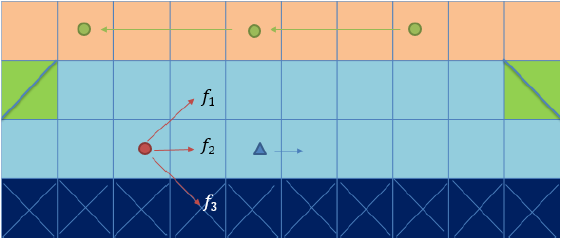
\includegraphics[width=0.7\textwidth]{social-forces}
 \caption[\enquote{Social Forces} für Grid-Zellen]{Vorschlag der \enquote{Social Forces} für Grid-Zellen (Fahrzeug auf Normalspur), aus \cite{dat-ba}}
 \label{figure:social-forces}
\end{figure}
\noindent
Von den ein Fahrzeug umgebenden acht Zellen müssen, aufgrund der Bewegungsrichtung, nur die drei betrachtet werden, die sich in Fahrtrichtung befinden.

Die Kräfte der Zellen, siehe \cref{figure:social-forces}, werden für jedes Fahrzeug zu jedem Zeitschritt $t$, da dessen Position zum Zeitpunkt $t + 1$ von der Position im vorhergehenden Zeitschritt abhängt, über verschiedene Funktionen berechnet. Das betrachtete Fahrzeug (Ego) befindet sich:
\begin{itemize}
	\item auf der Hauptspur 
	\begin{itemize}
		\item $f_{1}(a,v,\lambda) = \e^{\lambda(1-\frac{a}{v+\xi})}$ 
		\item $f_{2}(a,v,\lambda) = \frac{a}{\lambda(v+0,1)}$ 
		\item $f_{3} = 0$ 
	\end{itemize}
Hierbei ist $a$ der Abstand zum vorausfahrenden Fahrzeug, $v$ die relative Geschwindigkeit zwischen Ego und dem vorausfahrenden Fahrzeug und $\lambda$ ein Skalierungsfaktor. $\xi$ ist ein sehr kleiner positiver Wert, der die Durchführbarkeit der Division im Falle von $v=0$ sicherstellen soll. Für $f_{3}$ gibt es keinen Wert zu berechnen, da sich dort der Standstreifen befindet, der nicht befahren werden kann.
	\item auf der Überholspur 
	\begin{itemize}
		\item $h_{1} = 0$ 
		\item $h_{2}(a^{\prime},v^{\prime},\lambda) = \frac{v^{\prime}}{\lambda(a^{\prime}+0,1)}$ 
		\item $h_{3}(a^{\prime},v^{\prime},\lambda) = \e^{\lambda(1-\frac{v^{\prime}}{a^{\prime}+\omega})}$ 
	\end{itemize}
Hierbei ist $a^{\prime}$ der relative Abstand zum vorausfahrenden Fahrzeug auf der Hauptspur, $v^{\prime}$ die relative Geschwindigkeit zwischen Ego und dem vorausfahrenden Fahrzeug auf der Hauptspur und $\lambda$ auch hier der Skalierungsfaktor. $\omega$ entspricht $\xi$, im Fall dass $v^{\prime}=0$. Für $h_{1}$ wird kein Wert berechnet, da sich bei Betrachtung einer zweispurigen Fahrbahn in dieser Richtung keine weitere Spur in Fahrtrichtung befindet.
\end{itemize}

Die letztendliche Auswahl der Zielzelle für einen \enquote{Impuls zur Spurwahl} wird mittels \enquote{Fit\-ness-proportionate Selection} durchgeführt.

%%%%%

\subparagraph{\enquote{Fitness-proportionate Selection} oder \enquote{Roulette-wheel sampling}}

Die Konzept der \enquote{Fitness-proportionate Selection} kommt aus dem Bereich der genetischen Algorithmen. 
\cite{gen-algo} beschreibt es in einem Beispiel anhand einer Population von $n=4$ Strings, die man repräsentativ auch als Individuen oder Wahlmöglichkeiten ansehen kann. 
Jedem dieser Strings ist ein Funktionswert $f$ (Fitnesswert), ein Maß für Profit, Nutzwert oder Güte zugeordnet, den es zu maximieren gilt. 
Strings mit einem höheren Fitnesswert haben eine höhere Wahrscheinlichkeit, einen oder mehrere Nachkommen für die Folgegeneration beizutragen.
Demnach ist dies eine künstliche Version des Darwin'schen \enquote{Survival of the Fittest}.

\begin{table}[ht]
\begin{center}
\setlength{\tabcolsep}{0.5em} % for the horizontal padding
{\renewcommand{\arraystretch}{1.2}% for the vertical padding
\begin{tabular}{| l  c  c |}
\hline 
No. & Fitnesswert $f$ & \% von Gesamt \\ \hline 
1 & 169 & 14,4 \\ 
2 & 576 & 49,2 \\ 
3 & 64 & 5,5 \\ 
4 & 361 & 30,9 \\ \hline
Gesamt & 1170 & 100,0 \\ \hline
\end{tabular}
}
\caption{Beispiel nach \cite[Table 1.1]{gen-algo}}
\label{tab:beispiel-tabelle-roulette}
\end{center}
\end{table}

Ein einfacher Weg \textit{Fitness-proportionate Selection} zu veranschaulichen ist \textit{Roulette-wheel sampling}. 
Dabei wird jeder Option ein Bereich (Slot) auf einem Rouletterad zugewiesen, welcher von der Größe her deren Fitnesswert entspricht, siehe \cref{figure:meta-chart}. 

\begin{figure}[hptb]
 \centering
 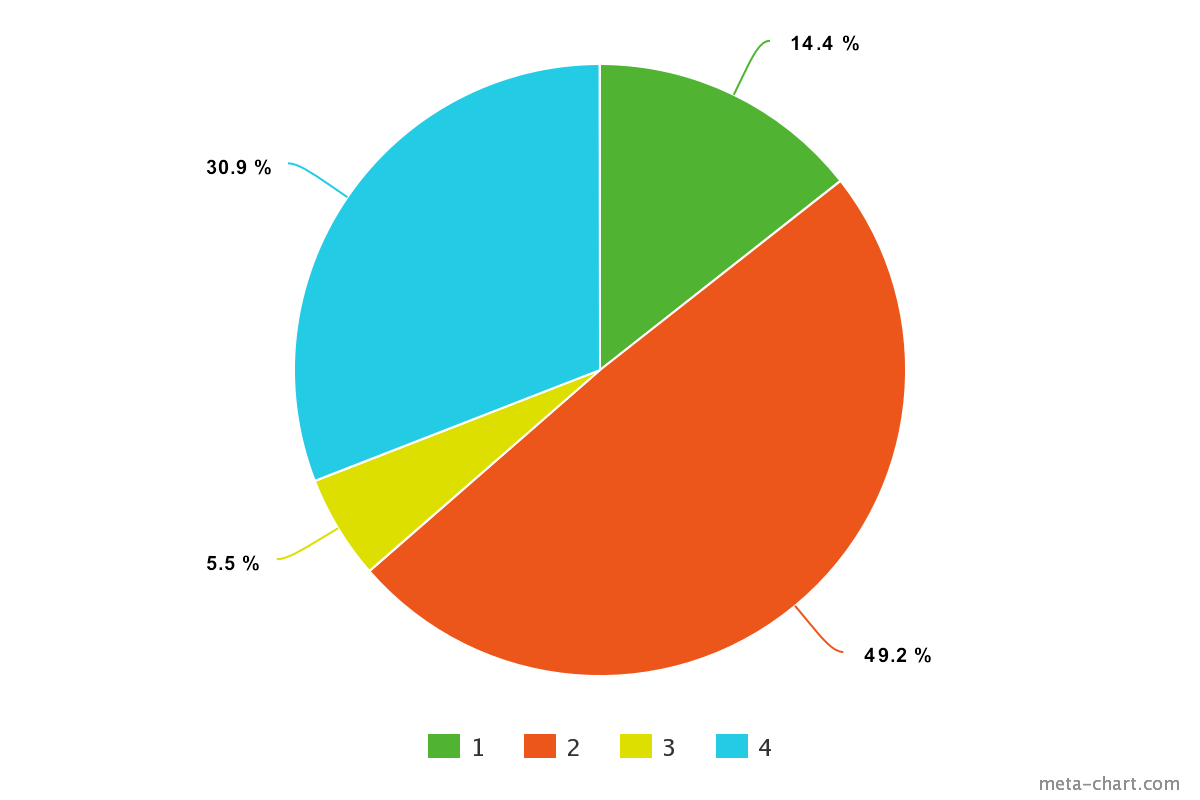
\includegraphics[width=0.7\textwidth]{meta-chart}
 \caption[gewichtetes Roulette-Rad (fitness-proportionate selection]
 		{schematische Darstellung eines gewichteten Rouletterades für der Beispiel in \cref{tab:beispiel-tabelle-roulette}}
 \label{figure:meta-chart}
\end{figure}

Benötigt man z. B. auch in der Nachfolgegeneration vier Strings, würde das Rouletterad viermal gedreht.
Das Individuum in dessen Slot die Kugel liegen bleibt, würde ausgewählt.

Aufgrund der Größe der Slots von String 2 und String 4 ist es z. B. möglich, dass String 2 für die Kindgeneration zweimal und String 4 gar nicht ausgewählt wird.

%%%%%

\subparagraph{Verwendung im Social-Force-Vehicle-Modell}

Im Social-Force-Vehicle-Modell gibt es zwei Möglichkeiten, aus denen gewählt werden kann. 
Zum einen jeweils das Geradeausfahren, zum anderen die Möglichkeit aus- respektive einzuscheren.
Für die Wahl der Alternative ist nur eine Entscheidung zwischen den jeweils zwei Möglichkeiten nötig.

Entgegen des Zwangs zum Ausscheren oder einer vorgegebenen Wahrscheinlichkeit für das Einscheren in der mehrspurigen Version des Nagel-Schreckenberg-Modells wird eine stochastische Simulationsmöglichkeit der Neigung zum Spurwechsel aufgezeigt.
Es entsteht eine Ungewissheit, ob die wahrscheinlichste Alternative ausgewählt wird oder ob die andere, weniger wahrscheinliche, das Verhalten bestimmen wird. 

\subparagraph{Möglichkeit von Kollisionen im Social-Force-Vehicle-Modell}

Da Kollisionen im Modell durch Ausweichen verhindert werden sollen, aber die \enquote{Bremskomponente} aus dem Ursprungsmodell entfernt wurde, ist in bestimmten Situationen ein Auffahrunfall denkbar.



%Bereits seit den 1950er Jahren wurden strömungsdynamische Ansätze für die Simulation von Verkehrsflüssen entwickelt. 
%Außerdem gab es ab den 1980er Jahren auch boolsche Simulationsmodelle, die mit Gitter-Gas-Automaten Flüssigkeiten simulieren konnten.
%Anfang der 1990er wurde von Kai Nagel und Michael Schreckenberg in \cite{na-sch} ein Verfahren vorgestellt, welches Autobahnverkehr basierend auf Zellularautomaten modelliert. 
%
%\begin{quote}
%Ein zellulärer Automat ist eine regelmäßige Annordnung von Zellen. Jede Zelle kann eine endliche Zahl von Werten / Zuständen annehmen und hat eine  begrenzte Zahl von Nachbarzellen, die sie beeinflussen können. Das Muster des gesamten zellulären Automaten ändert sich in einzelnen Schritten, die durch eine Reihe von Übergangsregeln bestimmt werden, die für alle Zellen gelten. (aus \cite{cell-autom})
%\end{quote}
%
%\noindent
%Vereinfacht kann eine Fahrspur einer Straße als Aneinanderreihung vieler solcher Zellen gesehen werden. 
%Dies führt schließlich zu einer gridbasierten Simulationsumgebung. 
%In \cite{na-sch} wird die Rechenumgebung als eindimensionales Array mit $L$ Zellen definiert. 
%Jede der Zellen kann entweder von einem Fahrzeug belegt oder frei sein. 
%Eine Simulation in dieser Grid-Welt hat den Vorteil, dass die Erkenntnisse auf die reale Welt skaliert werden können. 
%Es wird eine Zelllänge von 7,5\nolinebreak[4] m angenommen (vgl. \cite[S. 2227]{na-sch}), was ungefähr dem beanspruchten Platz eines Pkw - von Fahrzeugfront zu Fahrzeugfront - in einer Stausituation entspricht (Fahrzeuglänge + Abstand). 
%Jedes Fahrzeug hat eine ganzzahlige Geschwindigkeit zwischen null und $v_{max}$.
%
%\begin{table}[ht]
%\begin{center}
%\setlength{\tabcolsep}{0.5em} % for the horizontal padding
%{\renewcommand{\arraystretch}{1.2}% for the vertical padding
%\begin{tabular}{| c | c | c |}
%\hline 
%$v^{sim}$ in $\frac{Zellen}{Zeitschritt}$ & $\widehat{=}$ $v^{real}$ in $\frac{m}{s}$ & $=$ in $\frac{km}{h}$ \\ \hline 
%$1$ & 7,5 & 27 \\ \hline
%$2$ & 15 & 54 \\ \hline
%$3$ & 22,5 & 81 \\ \hline
%$4$ & 30 & 108 \\ \hline
%$5$ & 37,5 & 135 \\ \hline
%$6$ & 45 & 162 \\ \hline
%\end{tabular}
%}
%\caption{Umrechnung Geschwindigkeiten Gridwelt $\rightarrow$ reale Welt}
%\end{center}
%\label{tab:umrechnung-zelle-kmh}
%\end{table}
%
%\noindent
%Die beobachtete Durchschittsgeschwindigkeit von 4,5 Zellen/Zeitschritt, der als eine Sekunde angenommen wird, entspricht etwa der einer Geschwindigkeit von 120 km/h (vgl. \cite[S. 2227]{na-sch}). 
%
%In \cite{na-sch} war es erstmals gelungen, Wechselwirkungen zwischen Fahrzeugen im Einspurfall darzustellen und u. a. das Entstehen von Staus, ohne dass ein Grund dafür vorlag, zu modellieren. 
%Mit drei Regeln, die auf jedes Fahrzeug gleichzeitig und gleichermaßen anzuwenden waren, wurde ein realistischer Verkehrsfluss generiert. 
%Die folgenden Regeln, die die Kollisionsfreiheit sichern, sind die Grundlage für die, heute als \enquote{Nagel-Schreckenberg-Modell} bekannte, Modellierung:
%
%\begin{itemize}
%\item \textit{Beschleunigung}: Solange ein Fahrzeug nicht seine max. Geschwindigkeit $v_{max}$ (Zellen/""Zeitschritt) erreicht hat und ein vorausfahrendes Fahrzeug weit genug entfernt ist, erhöht es die Geschwindigkeit um $1$, $v \rightarrow v+1$;
%\item \textit{Abbremsen}: Hat ein Fahrzeug ein anderes Fahrzeug $j$ Zellen vor sich, dann reduziert es die Geschwindigkeit auf $j-1$, $v \rightarrow j-1$;
%\item Zufallsgröße, auch \textit{\enquote*{Trödelwahrscheinlichkeit}}: Mit einer Wahrscheinlichkeit $p$ wird die Geschwindigkeit ($v > 0$) eines Fahrzeuges um $1$ reduziert, $v \rightarrow v-1$
%\end{itemize}
%
%\noindent
%Die Anweisungen werden in der angegebenen Reihenfolge - für alle Fahrzeuge gleichzeitig - ausgeführt und jedes Fahrzeug um die entsprechende Anzahl Zellen weiter gesetzt.
%
%Dehnt man dieses Modell aber auf mehrere Fahrspuren aus, stößt es an seine Grenzen, weil die Modellierung von Überholvorgängen, bzw. genauer gesagt für das \enquote{Ausscheren} und \enquote{Einscheren}, nicht Teil des ursprünglichen Modells ist. 
%\cite{multi-lane} liefert eine \enquote*{multi-lane}-Betrachtung, wobei die ursprünglichen drei Regeln durch weitere ergänzt wurden, die zum einen ein Auffahren des Nachfolgeverkehrs auf den Spurwechsler und zum anderen auch des die Spur wechselnden auf vorausfahrende Fahrzeuge verhindern. \\
%In der Betrachtung, ob die Aktualisierung der Fahrzeuge parallel oder sequentiell erfolgen soll, wurde erkannt, dass dies für das entwickelte Modell nur geringe Unterschiede macht, da die Rate der Spurwechsel mit den festgelegten Regeln eher gering ist. \\
%Gleichzeitig wurde auch beobachtet, dass Fahrzeuge nicht wieder von der Überholspur in die Normalspur wechselten. Dies wurde mit weiteren Regeln und einer Spurwechselwahrscheinlichkeit abgestellt. Eine weitere Kalibrierung des Modells wurde in einer Folgearbeit durchgeführt. \\
%Durch die Konstanthaltung der Anzahl generierter Fahrzeuge und die Veränderung der Systemgröße konnten verschiedene Verkehrsdichten simuliert werden.
%
%\cite{multi-lane} zeigt mehrere Diagramme. Eine Untersuchung von realen Spurwechselvorgängen ergab, dass eine Umkehr der Benutzungshäufigkeit der rechten und linken Spuren bei einem Verkehrsfluss $q_{12}$ von etwa 1200 (Fahrzeugen) pro Stunde auf beiden Spuren erfolgt.
%
%Die Simulation ergab, dass der Punkt, an dem beide Spuren gleichermaßen benutzt werden, deutlich unter dem Punkt liegt, an dem der maximale Verkehrsfluss erreicht wird, siehe \cref{figure:verkehrsfluss-spurnutzung}.
%
%\begin{figure}[hptb]
% \centering
% 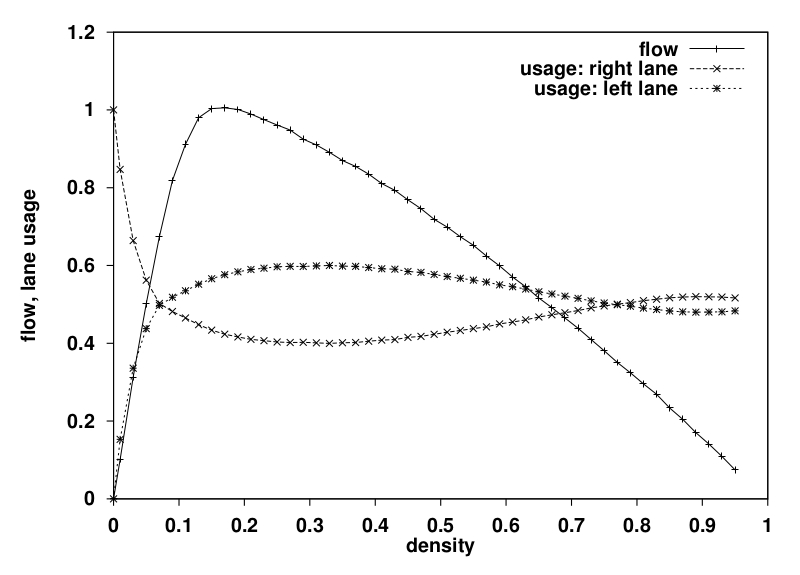
\includegraphics[width=0.7\textwidth]{verkehrsfluss-spurnutzung}
% \caption[Verkehrsfluss und Spurnutzung als Funktion der Verkehrsdichte]{Verkehrsfluss und Spurnutzung als Funktion der Verkehrsdichte, aus \cite{multi-lane}}
% \label{figure:verkehrsfluss-spurnutzung}
%\end{figure}
%
%\noindent
%Ein weiteres Resultat der Simulation ist eine mehrfache Umkehr der Nutzung der Fahrspuren abhängig von der Verkehrsdichte, wenn andere Parameter konstant gehalten werden, siehe \cref{figure:verkehrsfluss}.
%
%\begin{figure}[hptb]
% \centering
% 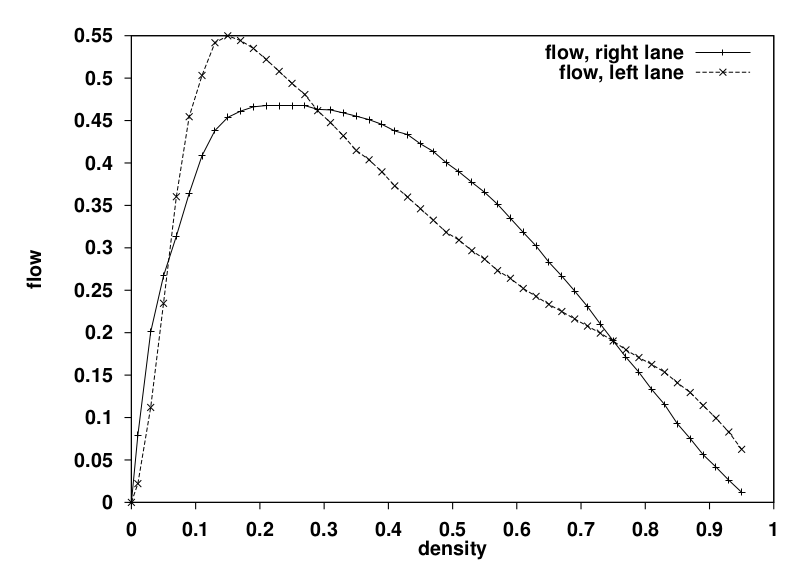
\includegraphics[width=0.7\textwidth]{verkehrsfluss}
% \caption[Verkehrsfluss als Funktion der durchschnittlichen Verkehrsdichte]{Verkehrsfluss auf den Fahrspuren als Funktion der durchschnittlichen Verkehrsdichte, aus \cite{multi-lane}}
% \label{figure:verkehrsfluss}
%\end{figure}
%
%\noindent
%Die Festlegung einer Wahrscheinlichkeit für das Zurückwechseln von der linken auf die rechte Fahrspur führte zu einer unterschiedlichen Spurwechselfrequenz, siehe \cref{figure:spurwechselfrequenz}.
%
%\begin{figure}[hptb]
% \centering
% 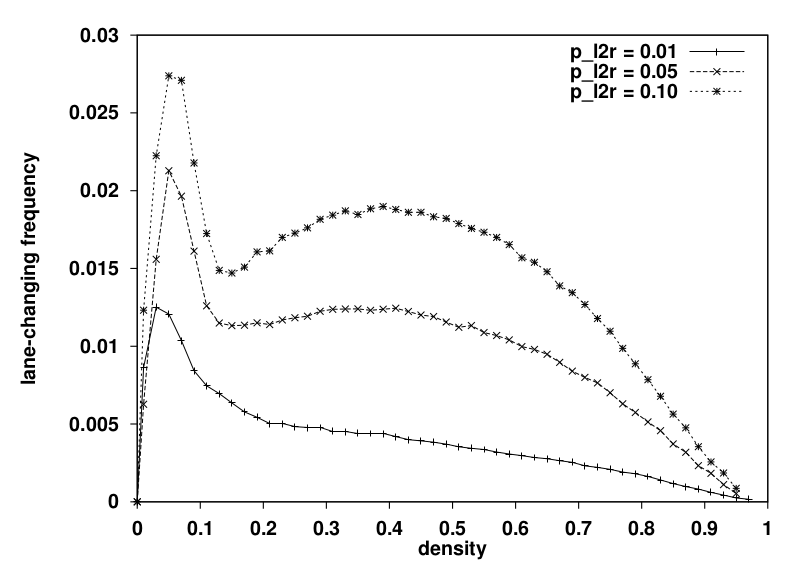
\includegraphics[width=0.7\textwidth]{spurwechselfrequenz}
% \caption[Spurwechselfrequenz als Funktion der Verkehrsdichte]{Spurwechselfrequenz als Funktion der Verkehrsdichte für verschiedene Spurwechselwahrscheinlichkeiten, aus \cite{multi-lane}}
% \label{figure:spurwechselfrequenz}
%\end{figure}
%
%\pagebreak
%In \cite{dat-ba} wurde mit dem \enquote{Social-Force-Vehicle-Modell} ein neuer Ansatz für die Simulation von Spurwechseln entwickelt.
%Auch hier wird eine Grid-Umgebung verwendet.
%Im Gegensatz zur ursprünglichen erdachten Nutzung der \enquote{Social Forces} für Fußgänger, wie z. B. in \cite{soc-for} beschrieben, wird dieses System auf die Gridzellen angewandt. Die Kräfte der Zellen, siehe \cref{figure:social-forces}, werden für jedes Fahrzeug zu jedem Zeitschritt $t$ berechnet, da seine Position zum Zeitpunkt $t + 1$ von der Position im vorhergehenden Zeitschritt abhängt.
%Von den ein Fahrzeug umgebenden acht Zellen müssen, aufgrund der Bewegungsrichtung, nur die drei betrachtet werden, die sich in Fahrtrichtung befinden.
%
%\begin{figure}[hptb]
% \centering
% 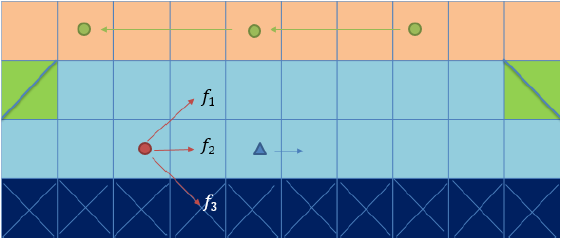
\includegraphics[width=0.7\textwidth]{social-forces}
% \caption[\enquote{Social Forces} für Grid-Zellen]{Vorschlag der \enquote{Social Forces} für Grid-Zellen, aus \cite{dat-ba}}
% \label{figure:social-forces}
%\end{figure}
%
%\noindent
%Die letztendliche Auswahl der Zielzelle wird mittels \enquote{Fitness-proportionate Selection} durchgeführt.
%Entgegen des Zwangs zum Ausscheren und einer fest vorgegebenen Wahrscheinlichkeit wird eine stochastische Simulationsmöglichkeit der Neigung zum Spurwechsel aufgezeigt.